%----------------------------------------------------------------------------------------
%	PACKAGES AND DOCUMENT CONFIGURATIONS
%----------------------------------------------------------------------------------------

\documentclass[12pt,a4paper]{article}

\usepackage[version=3]{mhchem} % Package for chemical equation typesetting
\usepackage{siunitx} % Provides the \SI{}{} and \si{} command for typesetting SI units
\usepackage{graphicx} % Required for the inclusion of images
\usepackage{natbib} % Required to change bibliography style to APA
\usepackage{amsmath} % Required for some math elements 
\usepackage{geometry}
\usepackage{enumerate}
\usepackage{float}
\usepackage{subfigure}
\usepackage{pdfpages}
\usepackage{siunitx}
\usepackage{fancyhdr}
\usepackage{textcomp}
\usepackage{gensymb}

\includepdfset{pagecommand={\thispagestyle{fancy}}}%page number for pdf

\renewcommand{\labelenumi}{\alph{enumi}.} % Make numbering in the enumerate environment by letter rather than number (e.g. section 6)
\geometry{left=2cm,right=2cm,top=3cm,bottom=3cm}

%\usepackage{times} % Uncomment to use the Times New Roman font

%----------------------------------------------------------------------------------------
%	DOCUMENT INFORMATION
%----------------------------------------------------------------------------------------


\begin{document}

\begin{center}
~\\
\rule[0mm]{400pt}{0.5pt}
\Large{ \textsc{\newline\\UM-SJTU Joint Institute\\Physics Laboratory\\(Vp241)\\}}
\rule[0mm]{400pt}{0.5pt}
\Large{ \textsc{\newline\newline\newline\newline\newline\newline\\
Laboratory Report\\}}
\Large{\textsc{ \\ Exercise 4  \\ Polarization of Light} }

\end{center}

\begin{description}
    \item[] 
    \item[] 
    \item[] 
    \item[] 
    \item[] 
    \item[]
    \item[]\qquad \qquad Name: Han Yibei \qquad ID:519370910123   \qquad    Group:11\\
    \item[]\qquad \qquad Date: \today
\end{description}

\newpage

%----------------------------------------------------------------------------------------
%	SECTION 1
%----------------------------------------------------------------------------------------
\section{Abstract}
In this experiment, the polarization phenomenon of light is studied and Malus' law is verified with the relative error -0.5\%; the way half-waveplate work, with $\Delta\theta$=$2\alpha$ and relative uncertainty 1.05\%; the way quarter-wave plates work in optical systems about the generation and detection of linearly, elliptically and circularly polarized light, when $\alpha=0\degree$, it's linearly polarized; when $\alpha=45\degree$, it's circularly polarized; when $\alpha=20\degree$, it's elliptically polarized; when $\alpha=70\degree$, we can verified what we observed at $\alpha=20\degree$. Calculations, figures and plots are used to  illustrate the result. Also, we discuss the uncertainty and possible error in this experiment.

\section{Introduction}
\subsection{Motivation}
The polarization of light played an important role in the development of wave optics. And there existed a wide range of applications in numerous areas, such as optical measurement techniques, crystal structure research, and experimental stress analysis.(Ref[1])

\subsection{Theoratical Background}
Light can be described as transverse electromagnetic waves, with the plane of oscillations perpendicular to the direction of light propagation. The natural light is a mixture of waves with random transverse directions, and it can also be called unpolarized light. The unpolarized light have the uniform distribution of the transverse directions.

\subsubsection{Polarization of Light}
Light vector describes a time-dependent, propagating electric field. The light vector maintains a certain oscillation direction, is called linearly polarized light and the line of the direction is called the polarization axis (Fig.5).\par 

\begin{figure}[H]
    \centering
    \includegraphics[width=7cm]{linearly.png}
    \caption{ (a) Linearly polarized light with the polarization axis perpendicular to the page plane. (b) Linearly polarized light with the polarization axis parallel to the page plane (Ref[1])}
    \label{linear}
\end{figure}

\begin{figure}[H]
    \centering
    \includegraphics[width=6cm]{elliptically.png}
    \caption{Elliptically xy plane polarized light propagating in the z direction (Ref[1])}
    \label{elliptically}
\end{figure}

The light with the light vector direction rotating and forms a circle with its endpoint, is called circularly polarized light. If the traces is an ellipse, the light is regarded as elliptically polarized (see Fig.\ref{elliptically}).\par 

Although natural light is unpolarized, it can be regarded as a mixture of linearly polarized waves with equal amplitudes and different transverse directions. The direction of partially polarized light is the same as the direction of the the light vector with maximum amplitude. \par


\subsubsection{Polarizer}
Polarizer is used to produce polarized light using the principle of dichroism, which can pass the light polarized in a certain direction while absorbed other light polarized in different directions. It helps generate linearly polarized light from natural light. (Ref[1])\par 
A polarization device can change incident natural light to polarized light (a polarizer), as well as detect and analyze dofferent type of polarized light (analyzer).

\subsubsection{Malus' Law}
The light coming out of a polarization device has change of the light brightness.

\begin{figure}[H]
    \centering
    \includegraphics[width=9cm]{makustheo.png}
    \caption{ Change in the brightness of the light depends on the mutual orientation of the polarizer and the analyzer.(Ref[1])}
    \label{brightnesschange}
\end{figure}

With two polarizers arranged parallel as the Fig.\ref{brightnesschange}, left one plays the role of a polarizer while other is an analyzer. Let the angle between their polarization axes be $\theta$. The light is incident normally on the polarizer and then continues to the analyzer. The intensity of the linearly polarized light leaving the analyzer is
\begin{equation}
    I_{light}=I_{light,0}cos^2\theta (Ref[1])
\end{equation}
where $I_{light}$ is the intensity of the linearly polarized light incident on the analyzer. \par
For a linearly polarized light, the transmitted light will change periodically when rotating the polarizer and will exist certain point when intensity is 0. For a elliptically or partially polarized light, the transmitted light will also change periodically. For the natural light and circularly polarized light, the intensity won't change at all. So er can distinguish the polarized light type from using the polarizer.

\subsubsection{Generation of Elliptically and Circularly Polarized Light. Half-wave and Quarter-wave Plates}
When linearly polarized light is incident on a crystal plate parallel to the optical axis, and the angle between the polarizing axis and the optical axis is $\alpha$. The linearly polarized light can be divide into two parts: an extraordinary wave with parallel oscillation direction pwith the optical axis and an ordinary wave with perpendicular direction with the optical axis. The final optical path difference over the thickness d is $\Delta=(n_e-n_o)d$ and the phase difference is
$$\delta=\frac{2\pi}{\lambda}(n_e-n_o)d (Ref[1])$$
where $\lambda$ is the wavelength, $n_e$ is the refractive index for the extraordinary axis, and $n_o$ is the refractive index for the ordinary axis.
\begin{figure}[H]
    \centering
    \includegraphics[width=5cm]{waveplate.png}
    \caption{Linearly polarized light passing through a waveplate.(Ref[1])}
    \label{waveplate}
\end{figure}

\begin{equation}
    \left\{
        \begin{aligned}
        &E_x=A_ocos\omega t \\
        &E_y=A_ocos(\omega t+\delta)
        \end{aligned}
    \right.
    \longrightarrow
    \frac{E_x^2}{A_o^2}+\frac{E_x^2}{A_o^2}-2\frac{E_xE_y}{A_oA_e}cos\delta=sin^2\delta (Ref[1])
\end{equation}
Some special cases can be discussed.\par 
When $\Delta=k\lambda$ (k=0,1,2,...), $\delta=0$. The equation is $E_y=\frac{A_e}{A_o}E_x$. The light through this kind of waveplate remain unchange and this kind of waveplate called full-wave plate.(Ref[1])\par
When $\Delta=(2k+1)\lambda/2$,(k=0,1,2...), and $\delta=\pi$. The equation is $E_y=-\frac{A_e}{A_o}E_x$. The light through it remain the same type but the axis rotate $2\alpha$. This kind of waveplant is called 1/2-wave plate.(Ref[1])\par 
When $\Delta=(2k+1)\lambda/4$ (k=0,1,2...), and $\delta=\pm\pi/2$. The equation is $\frac{E_x^2}{A_o^2}+\frac{E_y^2}{A_e^2}=1$. This kind of waveplate is called 1/4-wave plate. When $\alpha=0$ or $\pi/2$, the light is still linearly polarized. When $\alpha=\pi/4$, the transmitted life is circularly polarized. Otherwise, the transmitted light is elliptically polarized.(Ref[1]) \par 

\section{Discription of Experiment}
\subsection{Apparatus}
The measurement setup consists of: a semiconductor laser, a tungsten iodine lamp, a silicon photo-cell, a UT51 digital universal meter, as well as two polarizers, 1/2-wave and 1/4-wave plates (the uncertainty of the angle is 2°) and a lens with a glass sheet.(Ref[1])
The detailed information is shown in Table \ref{apparatus}.
\begin{table}[H]
    \centering
    \begin{tabular}{|c|c|}
    \hline
    \textbf{Apparatus} & \textbf{Uncertainty} \\ \hline
    Universal meter & $\pm$0.001$\mu$A \\ \hline
    Polarizer & $\pm$2\degree \\ \hline
    Analyzer  & $\pm$2\degree \\ \hline
    \end{tabular}
    \caption{Apparatus Information}
    \label{apparatus}
\end{table} 

\subsection{Measurement Procedure}
\subsubsection{Apparatus Adjustment}
At the beginning, we should choose the appropriate photo-cell aperture(see Fig) used in different experiments. And close the light to reduce uncertainty.
\begin{figure}[H]
    \centering
    \includegraphics[width=6cm]{photocell.jpg}
    \caption{Photo-cell(Ref[1])}
    \label{photocell}
\end{figure}
In this experiment, only the $\phi$6.0 aperture, which preserves the incident light intensity, is needed. Then adjust the laser and the photo-cell to enable the light pass through certain aperture. Also make sure that the light pass through the center of the lens and glass sheets between photo-cell and laser. Adjust the distance between the lens and the laser to make the light intensity in an appropriate range. Final adjustment step is to set the digital universal meter in the appropriate mode and range.

\subsubsection{Demonstration of Malus' Law}
Assemble the measurement setup as shown in Fig.\ref{apparatus}.First assemble the polarizer and check whether the present light is linearly polarized. Then put the analyzer on. Rotate the analyzer to find the maximum electric current $I_0$. Then, rotate the analyzer from 0\degree~to 90\degree, at the interval of 5\degree, record the magnitude of the current. Record the values plot the graph $I/I_0$ vs. $cos^2\theta$. Perform linear fitting and compare the data with the theoretical result.

\begin{figure}[H]
    \centering
    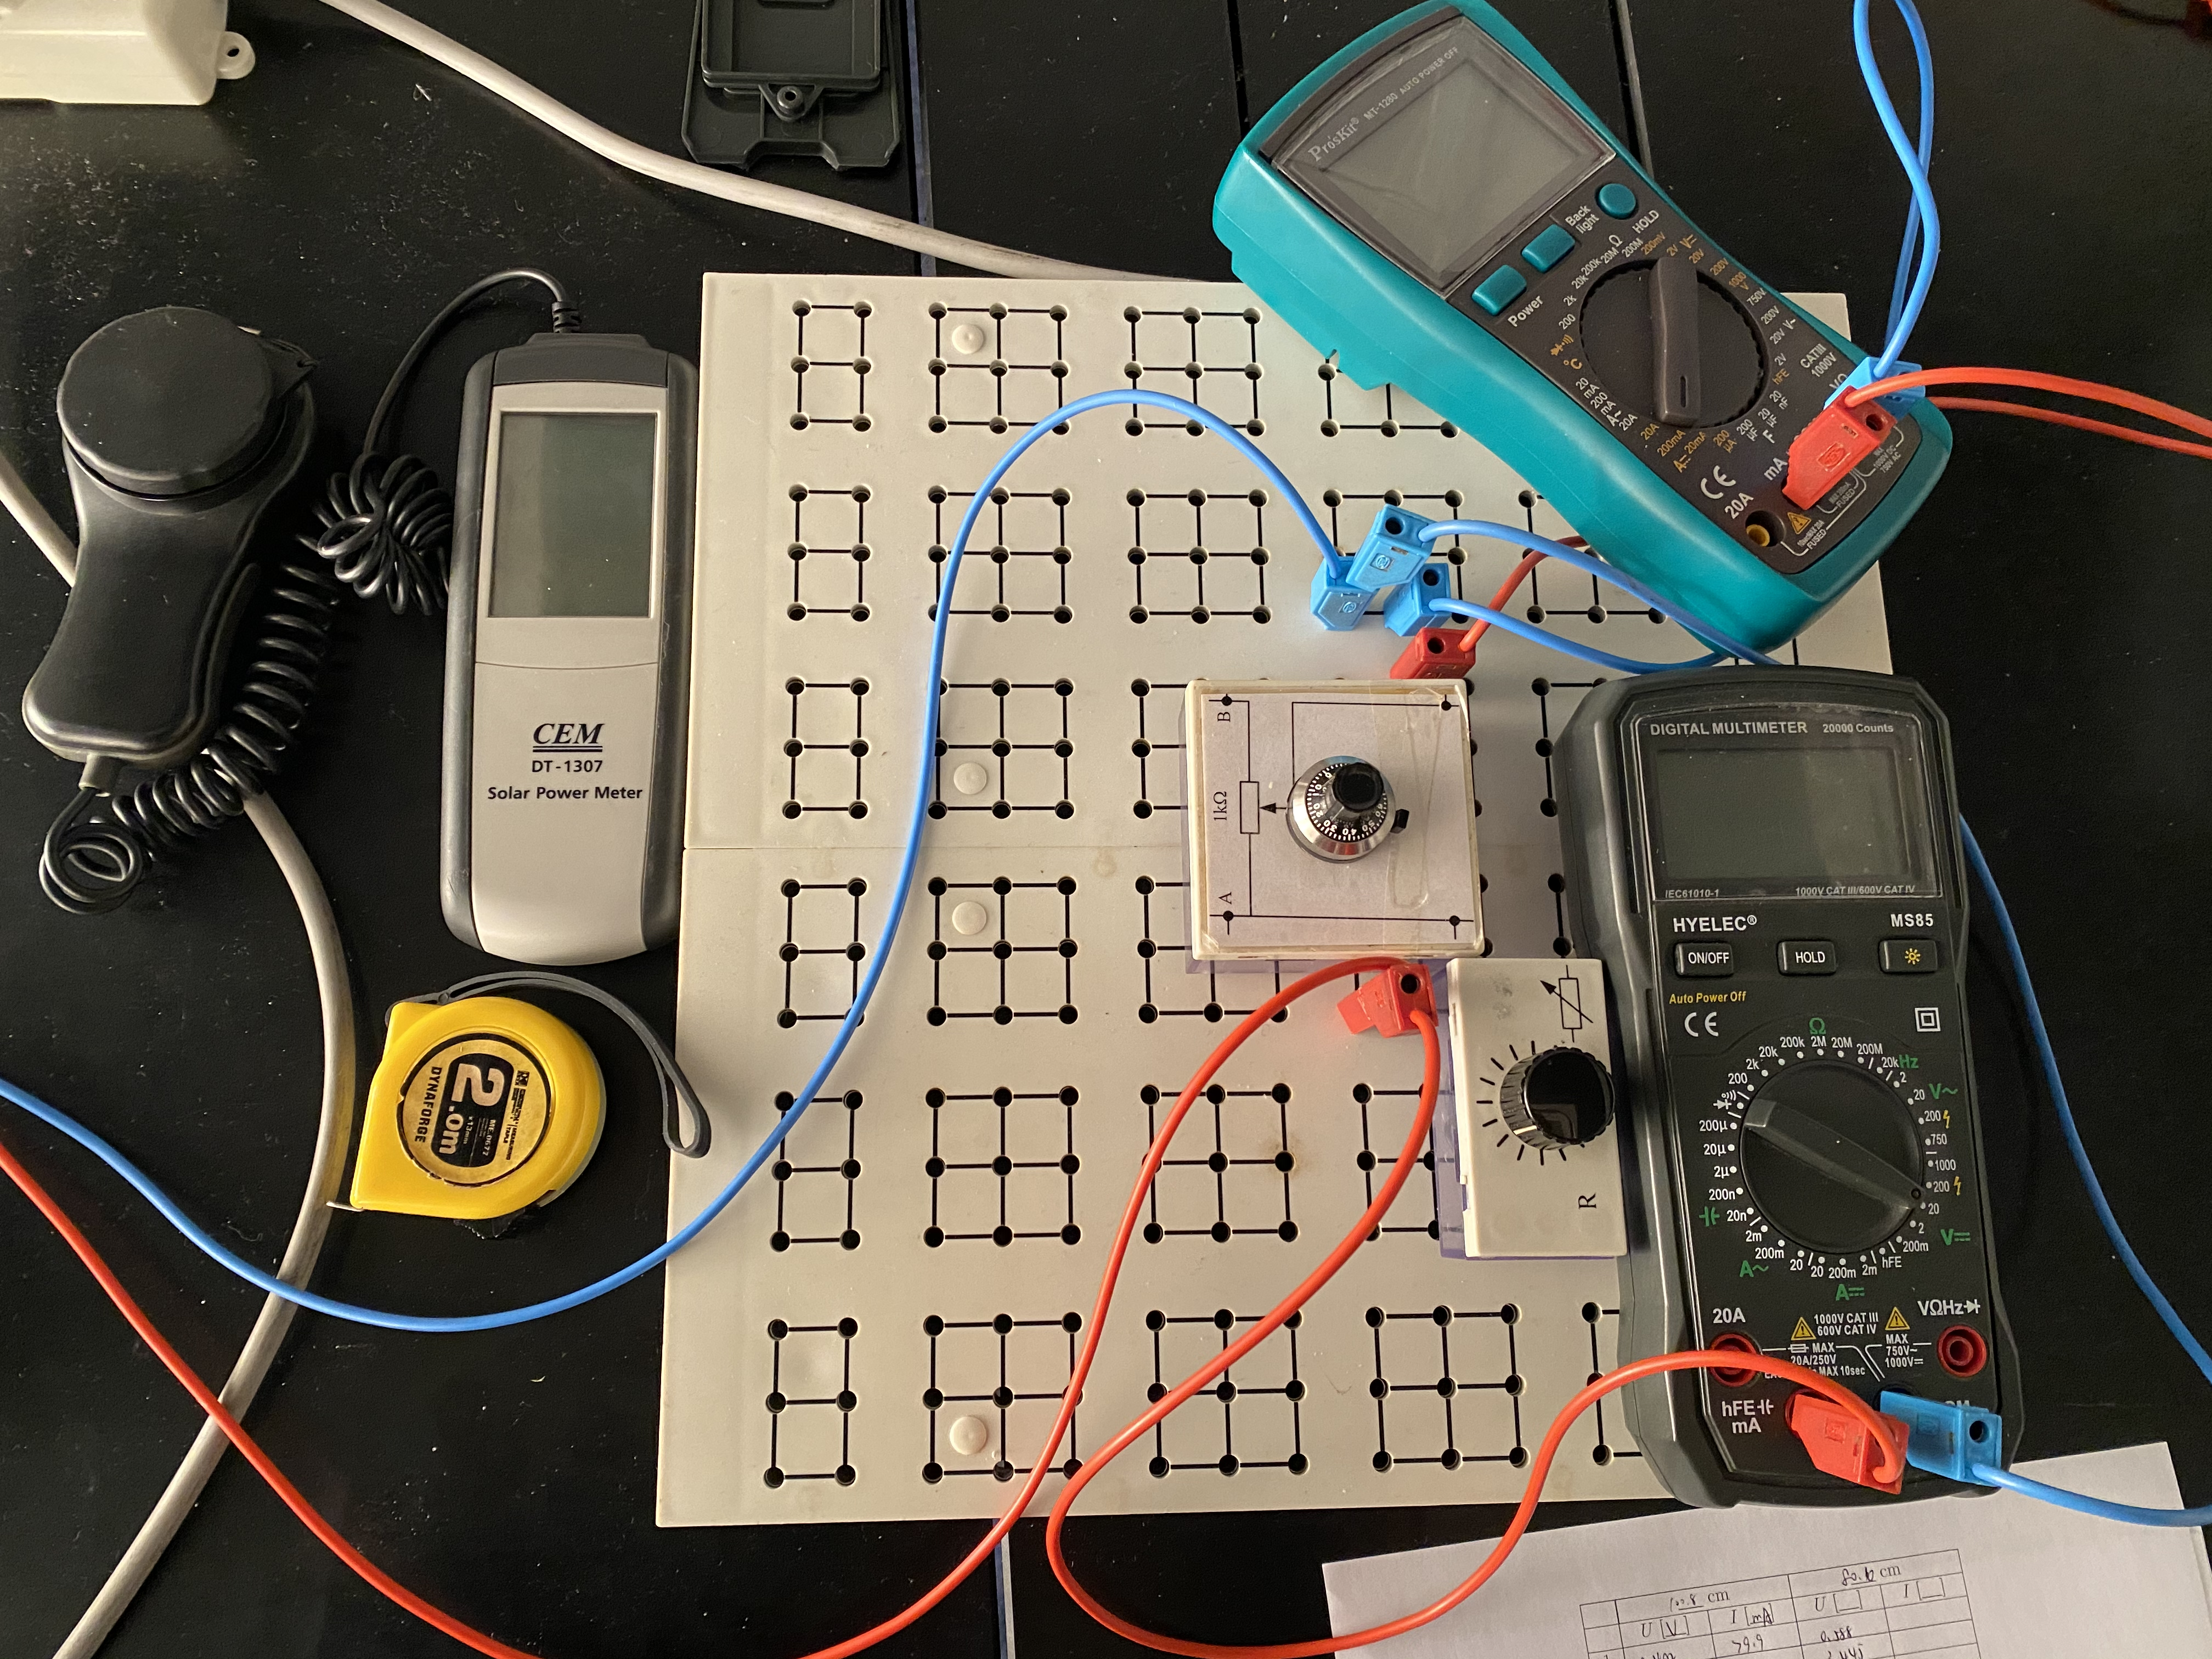
\includegraphics[width=7.5cm]{apparatus.jpg}
    \caption{Experimental setup for a demonstration of Malus' law.(Ref[1])}
    \label{apparatus}
\end{figure}

\subsubsection{Linearly Polarized Light and the Half-wave Plate}
\begin{figure}[H]
    \centering
    \includegraphics[width=7.5cm]{halfwave.png}
    \caption{Experimental setup for the 1/2-wave plate.(Ref[1])}
    \label{halfwave}
\end{figure}
Set up the equipment on the optical bench as shown in Fig.\ref{halfwave}. Make A and P perpendicular to each other before placing the half-wave plate. After inserting the half-wave plate, make the new extinction position as the reference position. Rotate the half-wave plate at the interval of 10\degree from the initial position, from 90\degree to 10\degree, then record $\Delta\theta$ in a table. Plot the graph $\Delta\theta$ vs. $\alpha$.

\subsubsection{Circularly and Elliptically Polarized Light and the 1/4-wave Plate}
Set up the equipment on the optical bench as shown in Fig.\ref{halfwave}7. Make A and P perpendicular to each other before placing the half-wave plate. After inserting the 1/4-wave plate, make the new extinction position as the reference position. Rotate the analyzer for 360° and record the light intensity for every 10°. Record the data in a table and also record the maximum intensity I0. Repeat for $\alpha$=20\degree, 45\degree. For $\alpha$=70\degree, just recording the maxium intensity and its corresponding changed angle $\Delta\theta$. Use a computer to plot the relation between the rotation angle of the analyzer and the light amplitude in polar coordinates. Mark the position recorded in $\alpha=70$\degree and compare it with the data recorded in $\alpha=20$\degree.

\subsubsection{Caution}
Do not direct the laser beam into the eye.
Do not touch the surface of the polarizers or the wave plates.
Please leave the equipment in order before leaving.

\section{Result}
\subsection{Malus' Law Demonstration}
We want to find the relationship between $cos^2\theta$ and $I/I_0$. All the result and uncertainty is shown in Tabel \ref{Marlustable}. Then we apply linear fit to $I/I_0$ vs. $cos^2\theta$, shown in Fig.\ref{malusfigure}.
\begin{figure}[H]
    \centering
    \includegraphics[width=12cm]{malus.png}
    \caption{Linear fit of $I/I_0$ vs. $cos^2\theta$}
    \label{malusfigure}
\end{figure}
From the figure we can see that the Pearson’s r is 0.999 and the intercept is close to 0, which means $I/I_0$ is proportional to $cos^2\theta$. The slope is $0.995\pm0.008$, and the theoretical value of the slope should be 1. The relative error is $u_r=\frac{0.995-1}{1}\times 100\%=-0.5\%$, which is very small.

\subsection{Linearly Polarized Light and the Half-wave Plate}
For the rotation angle of the analyzer, we need to perform the calculation, and the results and uncertainties is in Table \ref{changedata}.\par 
From the  we can see that the Pearson’s r is 0.999 which is very close to 1, and the intercept isvery close to 0. These mean that $\Delta\theta$ is proportional to $\theta$. The slope is $2.021\pm0.016$. The theoretical value of the slope should be 2(Ref[1]). The relative error is $u_r=(2.021-2)/2\times 100\%=1.05\%$, which is very small.\par
We can know from the procedure and the data that as the 1/2-wave plate rotates for 360\degree light extinction can be observed for 2 times. And after the linearly polarized light passes through the 1/2-wave plate with $\alpha$, the polarization axis will be rotated for $2\alpha$.

\begin{figure}[H]
    \centering
    \includegraphics[width=11cm]{change.png}
    \caption{Linear fit of $\Delta\theta$ vs. $\alpha$}
\end{figure}

\subsection{Circularly and Elliptically Polarized Light and the 1/4-wave Plate}
\subsubsection{Rotation angle 0\degree}
\begin{figure}[H]
    \centering
    \includegraphics[width=10.5cm]{0degree.png}
    \caption{Plot of $\sqrt{I/I_0}$ vs. $\theta$}
    \label{0degreefig}
\end{figure}
We want the relationship between $\sqrt{I/I_0}$ and $\theta$, we calculate all the result, shown in Table \ref{0degree}. Then we plot $\sqrt{I/I_0}$ vs. $\theta$ in the polar coordinate, shown in Fig.\ref{0degreefig}. 

\subsubsection{Rotation angle 20\degree}
We want the relationship between $\sqrt{I/I_0}$ and $\theta$, we calculate all the result, shown in Table \ref{20degree}. Then we plot $\sqrt{I/I_0}$ vs. $\theta$ in the polar coordinate, shown in Fig.\ref{20degreefig}.
\begin{figure}[H]
    \centering
    \includegraphics[width=10.5cm]{20degree.png}
    \caption{Plot of $\sqrt{I/I_0}$ vs. $\theta$}
    \label{20degreefig}
\end{figure}

\subsubsection{Rotation angle 45\degree}
\begin{figure}[H]
    \centering
        \includegraphics[width=12cm]{45degree.jpg}
        \caption{Plot of $\sqrt{I/I_0}$ vs. $\theta$}
        \label{45degreelinearfig}
\end{figure}

We want the relationship between $\sqrt{I/I_0}$ and $\theta$, we calculate all the result, shown in Table \ref{45degreelinearfig}. Then we plot $\sqrt{I/I_0}$ vs. $\theta$ in the polar coordinate, shown in Fig.\ref{45degreelinearfig}. The slope is 1.3447E-4, is very closed to 0. But the Pearson's r is relatively small, the reason will be discussed in conlusion part.


\subsubsection{Rotation angle 70\degree}
When the current reaches its maximum, we recorded the angle of the analyzer and the current in Table \ref{70degree}.
We also mark the maximum current point on the previous plot of 1/4-wave plate of the rotation angle 20\degree, shown in Fig.\ref{70degreefig}.
\begin{figure}[H]
    \centering
    \includegraphics[width=12cm]{70degree.png}
    \caption{Marked position}
    \label{70degreefig}
\end{figure}

\section{Conclusions}
\subsection{Conclusions}
In this lab, we understand some properties of light. Particularly, we study the polarization phenomenon and verify Malus' law, as well as understand the way half- and quarter-wave plates work in optical systems. Generation and detection of elliptically and circularly polarized light are also be investigated.
\subsubsection{Malus’ Law} 
We apply linear fit to $I/I_0$ vs. $cos^2\theta$. The result shows that the Pearson’s r is very close to 0 and the intercept is close to 1, which means $I/I_0$ is proportional to $cos^2\theta$. The slope is is very close to the theoretical value 1, with the relative error -0.5\%.\par 
From the result we verify Malus’ Law: $I _{light}=I _{light,0}\cdot cos^2 \theta$.
\subsubsection{Linearly Polarized Light}
We apply linear fit to $\Delta\theta vs. \theta$.The result shows that the Pearson’s r is very close to 1, and the intercept is very close to 0. These mean that $\Delta\theta$ is proportional to $\theta$. The slope is very close to the theoretical value 2(Ref[1]) with the relative error 1.05\%.\par 
This means that the polarization axis of a polarized light passing through the half-wave plate is rotated by an angle $2\alpha$ .


\subsubsection{Circularly and Elliptically Polarized Light}
\paragraph{5.1.3.1 Wave-plate Rotation angle=0\degree}~{} \newline
Observing the polar plot of $\sqrt{I/I_0}$ vs. $\theta$, we can see that there are two maximum light intensity near $\theta$=0\degree and $\theta$=180\degree and two light extinction near $\theta$=90\degree and $\theta$=270\degree. Since the minimum intensity is zero, so in this case, the transmitted light is linearly polarized. Its polarization axis is parallel to the optical axis of the 1/4-wave plate.
\paragraph{5.1.3.2 Wave-plate Rotation angle=20\degree}~{} \newline
Observing the polar plot of $\sqrt{I/I_0}$ vs. $\theta$, we can see that there are two maximum light intensity near $\theta$=110\degree and $\theta$=290\degree and two light intensity minimums near $\theta$=20\degree and $\theta$=200\degree, In this case, the transmitted light is elliptically polarized.
\paragraph{5.1.3.3 Wave-plate Rotation angle=45\degree}~{} \newline
Observing the polar plot of $\sqrt{I/I_0}$ vs. $\theta$, there is no light extinction, and the maximum and minimum light intensity are about the same. When $\theta$ is changing, the light intensity changes slightly. In this case, the transmitted light is circularly polarized.
\paragraph{5.1.3.4 Wave-plate Rotation angle=70\degree}~{} \newline
$$For~\alpha=\theta~\frac{E_x}{A_o^2}+\frac{E_y^2}{A_e^2}=1~(|cos\theta|>|sin\theta|) ~~max~at~90\degree$$ 
$$For~\alpha=90\degree-\theta~ \frac{E_x}{A_o^2}+\frac{E_y^2}{A_e^2}=1~(|cos\theta|>|sin\theta|) ~~max~at~0\degree$$ 
$$Angle~between~max=|\theta+\theta_{max\theta}+(90\degree-\theta)+\theta_{max(90\degree-\theta)}|=180\degree$$
Observing the marked position on Fig.\ref{70degreefig}, we find that the $\theta$ of red spot and the maximum spot of 20\degree and 70\degree has the sum of about 184\degree. $u_r=\frac{184-180}{180}\times 100\%=2.2\%$. From the equation above we can see that the two maximum current should be the same since the two elliptical has the same long axis. But there exit certain error in the experimrnt, the reason will be discussed in next error analysis part.\par 
We conclude that when rotation angles are complementary, the position where the light intensity reaches its maximum have the sum about 180\degree. The maximum light intensity is almost the same. \par




\subsection{Error Analysis}
\begin{itemize}
    \item Environment light will largely affect the result of this experiment.
    \item It is hard to make sure that the light passes through the center of the lens.
    \item We cannot ensure that the light is incident normally on the polarizer and the analyzer.
	\item The readings of the universal meter are unstable. The same angle may not result in the same light intensity at a second time.
	\item The uncertainty of the angle is relatively large.
	\item There are fingerprints and other stains on the surface of the plate and analyzer, which may cause error when the light is polarized. 
	\item Since the light intensity is indirectly found by measuring the electric current, there might be errors in the process of transforming the two factors.
	\item The class instructor came in and touched the laser beam, so the light intensity will be slightly changed, thus causing the difference between the maximum intensity in 70\degree and 20\degree.
\end{itemize}
	

\subsection{Improvements}
\begin{itemize}
    \item Do this experiment in a completely dark environment.
    \item Use digital device to record the angle of the analyzer, so that the uncertainty of the angle can be reduced.
\end{itemize}

\section{Reference}
\begin{enumerate}[1.]
    \item Jiang Shaopeng, Qin Tian, Cao Jianjun, Lin Xinyu, Zhong Xiaoxue, Mateusz Krzyzosiak, M. Krzyzosiak (2019). Exercise 4 - lab manual [rev. 5].pdf Shanghai: UMJI-SJTU.
\end{enumerate}


\newpage
{\LARGE\textbf{APPENDIX}}
\setcounter{section}{0}
\renewcommand\thesection{\Alph{section}}
\section{Data Table}
\begin{table}[H]
    \centering
    \begin{tabular}{|c|c|c|c|c|c|}
    \hline
    $\theta$[\degree]$\pm$2[\degree] & I[$\mu A$]$\pm$0.001$\mu A$      & $I/I_0$   & $u_{I/I_0}$       & $cos^2\theta$   &  $u_{cos^2\theta}$     \\ \hline
    0  & 0.738 & 1.0000 & 0.0008 & 1.000 & 0.000 \\ \hline
    5  & 0.729 & 0.9878 & 0.0008 & 0.992 & 0.006 \\ \hline
    10 & 0.715 & 0.9688 & 0.0008 & 0.970 & 0.012 \\ \hline
    15 & 0.690 & 0.9350 & 0.0008 & 0.933 & 0.017 \\ \hline
    20 & 0.661 & 0.8957 & 0.0008 & 0.88  & 0.02  \\ \hline
    25 & 0.612 & 0.8293 & 0.0008 & 0.82  & 0.03  \\ \hline
    30 & 0.555 & 0.7520 & 0.0008 & 0.75  & 0.03  \\ \hline
    35 & 0.501 & 0.6789 & 0.0008 & 0.67  & 0.03  \\ \hline
    40 & 0.446 & 0.6043 & 0.0008 & 0.59  & 0.03  \\ \hline
    45 & 0.380 & 0.5149 & 0.0008 & 0.50  & 0.03  \\ \hline
    50 & 0.317 & 0.4295 & 0.0007 & 0.41  & 0.03  \\ \hline
    55 & 0.253 & 0.3428 & 0.0007 & 0.33  & 0.03  \\ \hline
    60 & 0.192 & 0.2602 & 0.0007 & 0.25  & 0.03  \\ \hline
    65 & 0.141 & 0.1911 & 0.0007 & 0.18  & 0.03  \\ \hline
    70 & 0.095 & 0.1287 & 0.0007 & 0.12  & 0.02  \\ \hline
    75 & 0.057 & 0.0772 & 0.0007 & 0.067 & 0.017 \\ \hline
    80 & 0.026 & 0.0352 & 0.0007 & 0.030 & 0.012 \\ \hline
    85 & 0.008 & 0.0108 & 0.0007 & 0.008 & 0.006 \\ \hline
    90 & 0.000 & 0.0000 & 0.0007 & 0.000 & 0.000 \\ \hline
    \end{tabular}
    \caption{Calculation of $cos^2\theta$ and I/I0}
    \label{Marlustable}
\end{table}

\begin{table}[H]
    \centering
    \begin{tabular}{|c|c|c|c|}
    \hline
    $\alpha$  & $u_\alpha$     &  $\Delta\theta$   &  $u_{\Delta\theta}$    \\ \hline
    0  & 2.00 & 0   & 2.83 \\ \hline
    10 & 2.00 & 20  & 2.83 \\ \hline
    20 & 2.00 & 40  & 2.83 \\ \hline
    30 & 2.00 & 60  & 2.83 \\ \hline
    40 & 2.00 & 82  & 2.83 \\ \hline
    50 & 2.00 & 101 & 2.83 \\ \hline
    60 & 2.00 & 121 & 2.83 \\ \hline
    70 & 2.00 & 142 & 2.83 \\ \hline
    80 & 2.00 & 162 & 2.83 \\ \hline
    90 & 2.00 & 181 & 2.83 \\ \hline
    \end{tabular}
    \caption{Measurement data for the 1/2-wave plate}
    \label{changedata}
\end{table}

\begin{table}[H]
    \centering
    \begin{tabular}{|c|c|c|c|c|c|c|c|c|c|}
    \hline
    \multicolumn{10}{|c|}{Maximum Electric Current    $I_0$=0.500$\pm$0.001$\mu A$}       \\ \hline
    $\theta$ & $u_\theta$ &I& $\sqrt{I/I_0}$ & $u_{\sqrt{I/I_0}}$ &$\theta$ & $u_\theta$ &I& $\sqrt{I/I_0}$ & $u_{\sqrt{I/I_0}}$      \\ \hline
    0     & 2 & 0     & 0      & /      & 180   & 2 & 0     & 0      & /      \\ \hline
    10    & 2 & 0.013 & 0.161  & 0.006  & 190   & 2 & 0.012 & 0.155  & 0.007  \\ \hline
    20    & 2 & 0.052 & 0.322  & 0.003  & 200   & 2 & 0.051 & 0.319  & 0.003  \\ \hline
    30    & 2 & 0.116 & 0.482  & 0.002  & 210   & 2 & 0.115 & 0.480  & 0.002  \\ \hline
    40    & 2 & 0.194 & 0.6229 & 0.0019 & 220   & 2 & 0.192 & 0.6197 & 0.0019 \\ \hline
    50    & 2 & 0.283 & 0.7523 & 0.0017 & 230   & 2 & 0.276 & 0.7430 & 0.0017 \\ \hline
    60    & 2 & 0.361 & 0.8497 & 0.0015 & 240   & 2 & 0.354 & 0.8414 & 0.0016 \\ \hline
    70    & 2 & 0.428 & 0.9252 & 0.0015 & 250   & 2 & 0.421 & 0.9176 & 0.0015 \\ \hline
    80    & 2 & 0.482 & 0.9818 & 0.0014 & 260   & 2 & 0.466 & 0.9654 & 0.0014 \\ \hline
    90    & 2 & 0.499 & 0.9990 & 0.0014 & 270   & 2 & 0.485 & 0.9849 & 0.0014 \\ \hline
    100   & 2 & 0.48  & 0.9798 & 0.0014 & 280   & 2 & 0.473 & 0.9726 & 0.0014 \\ \hline
    110   & 2 & 0.438 & 0.9359 & 0.0015 & 290   & 2 & 0.428 & 0.9252 & 0.0015 \\ \hline
    120   & 2 & 0.378 & 0.8695 & 0.0015 & 300   & 2 & 0.365 & 0.8544 & 0.0015 \\ \hline
    130   & 2 & 0.292 & 0.7642 & 0.0016 & 310   & 2 & 0.285 & 0.7550 & 0.0017 \\ \hline
    140   & 2 & 0.207 & 0.6434 & 0.0018 & 320   & 2 & 0.203 & 0.6372 & 0.0019 \\ \hline
    150   & 2 & 0.127 & 0.504  & 0.002  & 330   & 2 & 0.124 & 0.498  & 0.002  \\ \hline
    160   & 2 & 0.063 & 0.355  & 0.003  & 340   & 2 & 0.058 & 0.341  & 0.003  \\ \hline
    170   & 2 & 0.018 & 0.190  & 0.005  & 350   & 2 & 0.017 & 0.184  & 0.006  \\ \hline
    \end{tabular}
    \caption{Calculation and Data of 0\degree~1/4-waveplate}
    \label{0degree}
\end{table}

\begin{table}[H]
    \centering
    \begin{tabular}{|c|c|c|c|c|c|c|c|c|c|}
    \hline
    \multicolumn{10}{|c|}{Maximum Electric Current $I_0=0.398±0.001\mu A$}       \\ \hline
    $\theta$ & $u_\theta$ &I& $\sqrt{I/I_0}$ & $u_{\sqrt{I/I_0}}$ &$\theta$ & $u_\theta$ &I& $\sqrt{I/I_0}$ & $u_{\sqrt{I/I_0}}$      \\  \hline
    0     & 2 & 0.076 & 0.437  & 0.003  & 180   & 2 & 0.078 & 0.443  & 0.003  \\ \hline
    10    & 2 & 0.049 & 0.351  & 0.004  & 190   & 2 & 0.049 & 0.351  & 0.004  \\ \hline
    20    & 2 & 0.041 & 0.321  & 0.004  & 200   & 2 & 0.041 & 0.321  & 0.004  \\ \hline
    30    & 2 & 0.055 & 0.372  & 0.004  & 210   & 2 & 0.055 & 0.372  & 0.004  \\ \hline
    40    & 2 & 0.089 & 0.473  & 0.003  & 220   & 2 & 0.092 & 0.481  & 0.003  \\ \hline
    50    & 2 & 0.137 & 0.587  & 0.002  & 230   & 2 & 0[1]43 & 0.599  & 0.002  \\ \hline
    60    & 2 & 0.198 & 0.705  & 0.002  & 240   & 2 & 0.202 & 0.712  & 0.002  \\ \hline
    70    & 2 & 0.260  & 0.808  & 0.002  & 250   & 2 & 0.265 & 0.816  & 0.002  \\ \hline
    80    & 2 & 0.312 & 0.8854 & 0.0019 & 260   & 2 & 0.312 & 0.8854 & 0.0019 \\ \hline
    90    & 2 & 0.353 & 0.9418 & 0.0018 & 270   & 2 & 0.356 & 0.9458 & 0.0018 \\ \hline
    100   & 2 & 0.386 & 0.9848 & 0.0018 & 280   & 2 & 0.385 & 0.9835 & 0.0018 \\ \hline
    110   & 2 & 0.397 & 0.9987 & 0.0018 & 290   & 2 & 0.396 & 0.9975 & 0.0018 \\ \hline
    120   & 2 & 0.378 & 0.9746 & 0.0018 & 300   & 2 & 0.375 & 0.9707 & 0.0018 \\ \hline
    130   & 2 & 0.343 & 0.9283 & 0.0018 & 310   & 2 & 0.342 & 0.9270 & 0.0018 \\ \hline
    140   & 2 & 0.296 & 0.8624 & 0.0019 & 320   & 2 & 0.293 & 0.8580 & 0.0019 \\ \hline
    150   & 2 & 0.235 & 0.768  & 0.002  & 330   & 2 & 0.238 & 0.773  & 0.002  \\ \hline
    160   & 2 & 0.177 & 0.667  & 0.002  & 340   & 2 & 0.178 & 0.669  & 0.002  \\ \hline
    170   & 2 & 0.120  & 0.549  & 0.003  & 350   & 2 & 0.121 & 0.551  & 0.003  \\ \hline
    \end{tabular}
    \caption{Calculation and Data of 20\degree~1/4-waveplate}
    \label{20degree}
\end{table}

\begin{table}[H]
    \centering
    \begin{tabular}{|c|c|c|c|c|c|c|c|c|c|}
    \hline
    \multicolumn{10}{|c|}{Maximum Electric Current $I_0=0.211\pm0.001\mu A$}      \\ \hline
    $\theta$ & $u_\theta$ &I& $\sqrt{I/I_0}$ & $u_{\sqrt{I/I_0}}$ &$\theta$ & $u_\theta$ &I& $\sqrt{I/I_0}$ & $u_{\sqrt{I/I_0}}$     \\ \hline
    0     & 2 & 0.172 & 0.903 & 0.004 & 180   & 2 & 0.173 & 0.905 & 0.004 \\ \hline
    10    & 2 & 0.178 & 0.918 & 0.004 & 190   & 2 & 0.182 & 0.929 & 0.003 \\ \hline
    20    & 2 & 0.186 & 0.939 & 0.003 & 200   & 2 & 0.187 & 0.941 & 0.003 \\ \hline
    30    & 2 & 0.187 & 0.941 & 0.003 & 210   & 2 & 0.196 & 0.964 & 0.003 \\ \hline
    40    & 2 & 0.210  & 0.998 & 0.003 & 220   & 2 & 0.196 & 0.964 & 0.003 \\ \hline
    50    & 2 & 0.215 & 1.009 & 0.003 & 230   & 2 & 0.200   & 0.974 & 0.003 \\ \hline
    60    & 2 & 0.217 & 1.014 & 0.003 & 240   & 2 & 0.208 & 0.993 & 0.003 \\ \hline
    70    & 2 & 0.210  & 0.998 & 0.003 & 250   & 2 & 0.206 & 0.988 & 0.003 \\ \hline
    80    & 2 & 0.202 & 0.978 & 0.003 & 260   & 2 & 0.198 & 0.969 & 0.003 \\ \hline
    90    & 2 & 0.210  & 0.998 & 0.003 & 270   & 2 & 0.190  & 0.949 & 0.003 \\ \hline
    100   & 2 & 0.193 & 0.956 & 0.003 & 280   & 2 & 0.181 & 0.926 & 0.003 \\ \hline
    110   & 2 & 0.183 & 0.931 & 0.003 & 290   & 2 & 0.171 & 0.900 & 0.004 \\ \hline
    120   & 2 & 0.178 & 0.918 & 0.004 & 300   & 2 & 0.166 & 0.887 & 0.004 \\ \hline
    130   & 2 & 0.175 & 0.911 & 0.004 & 310   & 2 & 0.155 & 0.857 & 0.004 \\ \hline
    140   & 2 & 0.176 & 0.913 & 0.004 & 320   & 2 & 0.157 & 0.863 & 0.004 \\ \hline
    150   & 2 & 0.165 & 0.884 & 0.004 & 330   & 2 & 0.160  & 0.871 & 0.004 \\ \hline
    160   & 2 & 0.167 & 0.890 & 0.004 & 340   & 2 & 0.159 & 0.868 & 0.004 \\ \hline
    170   & 2 & 0.170  & 0.898 & 0.004 & 350   & 2 & 0.166 & 0.887 & 0.004 \\ \hline
    \end{tabular}
    \caption{Calculation and Data of 45\degree~1/4-waveplate}
    \label{45degree}
\end{table}

\begin{table}[H]
    \centering
    \begin{tabular}{|c|c|}
    \hline
     I$[\mu A]\pm0.001\mu A$& 0.317 \\ \hline
     $\theta$[\degree]$\pm$2\degree& 74    \\ \hline
     $\sqrt{I/I_0}$& 1.000  \\ \hline
     $u_{\sqrt{I/I_0}}$ & 0.002  \\ \hline
    \end{tabular}
    \caption{Calculation and Data of 70\degree 1/4-waveplate}
    \label{70degree}
\end{table}

\end{document}